\chapter{GameObject ``Player`` \& Komponenten}

Die Spielfigur, die der Anwender bedient stellte sich w"ahrend der Entwicklung als komplexestes GameObject heraus. In diesem Kapitel geben wir daher einen "Uberblick "uber die Realisierung mithilfe von Sprites sowie der verschiedenen anh"angenden und selbsterstellten Skripte

\begin{figure}
	\centering
	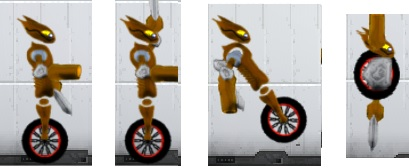
\includegraphics[height=5cm]{images/AnimationenZusammenschnitt.jpg}
	\caption{Zusammenschnitt der Player Sprites}
	\label{fig:playerSprites}
\end{figure}

\section{SpriteRenderer}

\section{AttributeComponent Skript}
Die AttributeComponent dient dazu die spielmechanischen Daten zu hinterlegen und zu verwalten. Sie kann sowohl dem Spieler als auch freundlich und feindlich Gesinnten NPCs angehängt werden. 

Nachfolgend werden die wichtigsten Daten vorgestellt:
\begin{lstlisting}[breaklines=true]
//Lebenspunkte, maximale Lebenspunkte, Ruestung und Schaden
public float health, maxHealth, armor, damage;
//Maximale Ausdauer, Ausdauer und regenerierte Ausdauer pro Sekunde
public float maxStamina, stamina, staminaPerSecond;
//Munition, Munitionskapazitaet und Reichweite
//Range = 0 -> Nahkampf / Range > 0 -> Fernkampf
public int ammo, ammoCap, range;
//Klon aktiv?
public bool cloneAlive = false;

//Cooldown für Plasmaschuss
static float cooldown1 = 1.0f;
//Laeuft cooldown für Plasmaschuss?
bool cooldown1Active = false;

//Cooldown fuer Klonfaehigkeit
static float cooldown2 = 10.0f;
//Time-to-live für Klon
static float ttl = 5.0f;
//Aktuelle Time-To-Live
float attl = ttl;
//Laeuft cooldown fuer Klon?
bool cooldown2Active = false;

//Referenz auf das Nahkampfsystem
MeleeSystem meleeSys;
\end{lstlisting}

Die Update-Funktion der AttributeComponent wird ausschlie"slich dazu benutzt, die Stamina "uber Zeit aufzuf"ullen w"ahrend die fixedUpdate-Funktion für das löschen des Klones verantwortlich ist.
\begin{lstlisting}[breaklines=true]
void Update () {

/*Fuelle Ausdauer ueber Zeit wieder auf solange maximalStamina nicht erreicht ist und die
Spielfigur sich nicht bewegt*/
if (staminaPerSecond > 0.0f && stamina < maxStamina && !meleeSys.animationRunning)
{
//Stelle sicher, dass Stamina nicht kleiner als 0 oder groesser als maximalStamina gesetzt wird
stamina = Mathf.Clamp(stamina+staminaPerSecond * Time.deltaTime,0,maxStamina);
}   
}
void FixedUpdate()
{
if (attl > 0)
attl -= Time.deltaTime;
if (attl <= 0 && cloneAlive)
{
Destroy(GameObject.Find("Klon"));
cloneAlive = false; 
}
}
\end{lstlisting}

\section{CharacterMovement Skript}



\section{MeleeSystem Skript}


\section{HealthSystem Skript}
